\documentclass[hyperref={pdfpagelabels=false}]{beamer}
% beamer already loads hyperref; do NOT load \usepackage{hyperref} again.

\usepackage{ragged2e} % 文字向兩邊對齊
\renewcommand{\raggedright}{\leftskip=0pt \rightskip=0pt plus 0cm}

\usepackage{listings}
\usepackage{lmodern}
\usepackage{fontspec}
\usepackage{xeCJK}
\setCJKmainfont{Noto Sans CJK TC}
%（可選）若你會用到無襯線中文或等寬中文，建議補上：
\setCJKsansfont{Noto Sans CJK TC}
\setCJKmonofont{Noto Sans Mono CJK TC}

\usepackage[english]{babel}
\usepackage{amsmath,amssymb,amsfonts,amsthm}

% hyperref settings (since beamer already loads hyperref)
\hypersetup{
  colorlinks=true,
  urlcolor=blue,
  citecolor=blue,
  pdfborder={0 0 0}
}

\usepackage{accsupp}% http://ctan.org/pkg/accsupp
\newcommand{\emptyaccsupp}[1]{\BeginAccSupp{ActualText={}}#1\EndAccSupp{}}

\usepackage{tikz}
\usetikzlibrary{arrows,decorations.pathmorphing,backgrounds,fit,positioning,shapes.symbols,chains}

\usepackage{booktabs}
\usepackage{threeparttable}
\usepackage{colortbl} 
\usepackage{xcolor}
\usetikzlibrary{tikzmark}

\newcommand{\indep}{\perp\!\!\!\perp}
\newcommand{\nindep}{\not\!\perp\!\!\!\perp}

\beamertemplatefootpagenumber


\usepackage{listings}
%%%%%%%%%%%%%%%%%%%%%%%%%%%%%%%%%%%%%%%%%%%%%%%%%%%%%%%%%%%%%%%%%%%%%%%%%%%%%%
% LaTeX snippet: language and style definition of Stata for listings package.
%                [listings](http://www.ctan.org/pkg/listings) 
%                [Stata](http://www.stata.com/)
%
% Usage:
%     Copy the code into your preamble, or import it by `\include` .
%     then in your doc:
%     \lstinputlisting[style=numbers]{DO-SCRIPT}
%     \lstinputlisting[style=numbers, style=stata-editor]{DO-SCRIPT}
%     \lstinputlisting[style=nonumbers, frame=none]{DO-SCRIPT}
% How it works:
%     - The language is defined by `\lstdefinelanguage{Stata}`
%     - Four styles is defined by `\lstdefinestyle{STYLE-NAME}`, 
%       they are: numbers and no numbers, plain(black and white) and colorful
%       (colored roughly like stata editor.)
% Tips:
%     - Generally you only need to set your default in the last part,
%       that is, code inside of `\lstset`.
%     - Add more keywords(I can not list all of them) in the `\lstset` part.
%     - Do NOT leave any blank lines in commands
%       (`\lstddefinelanguage', `\lstdefinestyle` and `\lstset`)
%
% update: 2014-04-16
% version: 0.1
% author: kongs
% licence: MIT
% url: https://gist.github.com/kongs-sublime/10862838
%
% TODO: 
%       - finish keyword list.
%       - precise colors that match stata editor?
%       - make it flexible(fonts and style)
%
%%%%%%%%%%%%%%%%%%%%%%%%%%%%%%%%%%%%%%%%%%%%%%%%%%%%%%%%%%%%%%%%%%%%%%%%%%%%%%


% langugae defination
\lstdefinelanguage{Stata}{
	% Left for users to add missing commands,
	% with possibility of choosing different style.
	morekeywords=,
	% Popular add-on commands
	morekeywords=[2]{cntrade, chinafin, 
		wbopendata, spmap,
	},
	% System commands
	morekeywords=[3]{regress, summarize, 
		display,
	},
	% Keywords
	morekeywords=[4]{forvalues, if, foreach, set},
	% Built-in functions
	morekeywords=[5]{rnormal, runiform},
	morecomment=[l]{//},
	% morecomment=[l]{*},  // `*` maybe used as multiply operator. So use `//` as line comment.
	morecomment=[s]{/*}{*/},
	% morecomment=[s]{,}{//},
	% The following is used by macros, like `lags'.
	morecomment=[n][keywordstyle9]{`}{'},
	morestring=[b]",
	sensitive=true,
}

\lstdefinestyle{numbers}{
	numbers=left, 
	stepnumber=1, 
	numberstyle=\tiny\emptyaccsupp,
	xleftmargin=2em,
}

\lstdefinestyle{nonumbers}{
	numbers=none,
}

\lstdefinestyle{stata-plain}{
	language=Stata,
	basicstyle=\footnotesize\ttfamily,
}

\lstdefinestyle{stata-editor}{
	language=Stata,
	basicstyle=\footnotesize\ttfamily,  
	keywordstyle={\color{NavyBlue}},  
	keywordstyle=[2]{\color{NavyBlue}},
	keywordstyle=[3]{\color{NavyBlue}},
	keywordstyle=[4]{\color{NavyBlue}},
	keywordstyle=[5]{\color{Blue}},
	keywordstyle=[9]{\color{TealBlue}},
	stringstyle=\color{Maroon},
	commentstyle=\color{OliveGreen},
}

\lstset{
	language=Stata,
	style=stata-plain,
	% style=stata-editor,
	style=numbers,
	showstringspaces=false,
	breaklines,
	frame=single,
	% To add missing commands
	% morekeywords={xtreg, xtunitroot},
}




\title[]  
{Fixed Effects Regression}


\author 
{Prof. Tzu-Ting Yang  \\ 楊子霆}

%\institute{Institute of Economics, Academia Sinica  \\ Econ, NTU}
\institute{Institute of Economics, Academia Sinica  \\ 中央研究院經濟研究所}
%\institute{Institute of Economics, Academia Sinica  \\ Econ, NTU}
%\institute{Institute of Economics, Academia Sinica  \\ IMES/IDAS, NCCU}

%\author 
%{楊子霆 \\ 中研院經濟所}

%\institute 
%{中正大學國際經濟專題研討}




\date
{\today}

% \usetheme{CambridgeUS}
% %\usecolortheme{seahorse}
% \setbeamertemplate{footline}{%
% 	\hfill\usebeamercolor[fg]{page number in head/foot}%
% 	\usebeamerfont{page number in head/foot}%
% 	\insertframenumber\,/\,\inserttotalframenumber\hspace{1em}\vspace{2pt}%
% }

% \usetheme{Boadilla}
% %\useinnertheme{rectangles}

% %\usetheme{CambridgeUS}
% \usecolortheme{seahorse}
% \setbeamertemplate{footline}{%
% 	\hfill\usebeamercolor[fg]{page number in head/foot}%
% 	\usebeamerfont{page number in head/foot}%
% 	\insertframenumber\,/\,\inserttotalframenumber\hspace{1em}\vspace{2pt}%
% }


%\usepackage{beamerthemeshadow}
%\usecolortheme{seahorse}
\setbeamertemplate{footline}{%
	\hfill\usebeamercolor[fg]{page number in head/foot}%
	\usebeamerfont{page number in head/foot}%
	\insertframenumber\,/\,\inserttotalframenumber\hspace{1em}\vspace{2pt}%
}


%\usepackage{beamerthemeshadow}

\beamersetuncovermixins{\opaqueness<1>{25}}{\opaqueness<2->{15}}

\begin{document}
	
	
	\begin{frame}{}
	\titlepage
\end{frame}





\begin{frame}{Observables and Unobservables Confounding Factors}
	\begin{itemize} 
		
		\item The main problem we face in estimating causal effect is that:
						\vspace{0.2cm}
			\begin{itemize} 
		\item Each individual, firm, state, or country can select treatment 
						\vspace{0.2cm}
						\begin{itemize} 			
		\item This choice could be correlated with factors that affect the outcomes of interest, which results in selection bias
						\vspace{0.2cm}
									\end{itemize}
			\end{itemize}
		\item So far the key strategy to obtain causal effect was to control for \textbf{observed} confounding factors
								\vspace{0.2cm}
		
		\item Yet, what if important confounding factors are unobserved?
		
		
		
		%\item Individuals with certain characteristics may be much more likely to be treated than others (selection bias)
		
		%\begin{equation*}
		%\mathrm{E}[\mathrm{Y}^{0}_{it} |D_{it}=1] \neq %\mathrm{E}[\mathrm{Y}^{0}_{it} |D_{it}=0]
		%\end{equation*}
		
	\end{itemize}
\end{frame}


\title[]  
{Main Idea}


\author 
{}

%\institute{Institute of Economics, Academia Sinica  \\ Econ, NTU}
%\institute{Institute of Economics, Academia Sinica  \\ IMES/IDAS, NCCU}
\institute{}

%\author 
%{楊子霆 \\ 中研院經濟所}

%\institute 
%{中正大學國際經濟專題研討}




\date
{}


\begin{frame}{}
	\titlepage
\end{frame}



\begin{frame}{Fixed Effects Regression}
	\begin{itemize} 
		
		\item If unobserved confounding factors are \textbf{time-invariant}
		\vspace{0.2cm}
		\begin{itemize} 
			
			
			\item If we have multiple time periods panel data or cross-sectional data
					\vspace{0.2cm}
			\item We can still obtain causal effect by estimating a regression that include many fixed effects in the model
			\vspace{0.2cm}
		\end{itemize}
	
		
		
		%\item Individuals with certain characteristics may be much more likely to be treated than others (selection bias)
		
		%\begin{equation*}
		%\mathrm{E}[\mathrm{Y}^{0}_{it} |D_{it}=1] \neq %\mathrm{E}[\mathrm{Y}^{0}_{it} |D_{it}=0]
		%\end{equation*}
		
	\end{itemize}
\end{frame}




\begin{frame}{Fixed Effects Regression}{Example}
	\begin{itemize} 
		\item Suppose we are interested in the question whether 
		joining union increase workers' earnings
		\vspace{0.2cm}
		\item We might want to estimate the following regression:
	
		\begin{equation*}
		Y_{it}=\delta+\alpha D_{it}+A'_i\gamma+X'_{it}\beta + \varepsilon_{it}
	\end{equation*}
	
		\begin{itemize} 
		\item $Y_{it}$ is outcome variable: earnings
				\vspace{0.2cm}
		\item $D_{it}$ is treatment variable: union status
					\vspace{0.2cm}
		\item $X_{it}$ are 	observed time-varying covariates: experience, education  
							\vspace{0.2cm}
		\item $A_i$	is unobserved but fixed confounder (time-invariant): ability or personality
		\vspace{0.2cm}
		\item Assume $E[\varepsilon_{it}|A_i,X_{it}]=0$				
			\end{itemize}	
	%	\item \textbf{Problem:} unionized workers may be different (e.g. higher skilled, more experienced) from non-unionized workers
	%	\vspace{0.2cm}
	%	\item Many of these factors will not be observable to the econometrician: \textbf{omitted variable bias}
		%	\vspace{0.2cm}
		%\item Therefore the error term and union status will be correlated and OLS will be biased.
	\end{itemize}
\end{frame}


\begin{frame}{Fixed Effects Regression}{Example}
	\begin{itemize} 
		\item This regression equation implies the following potential outcomes:
		
		\begin{equation*}
		Y^{0}_{it}=\delta+A'_i\gamma+X'_{it}\beta+ \varepsilon_{it}
		\end{equation*}
		
		
		\begin{equation*}
			Y^{1}_{it}=Y^{0}_{it}+ \alpha
		\end{equation*}
		
	\end{itemize}
\end{frame}







\begin{frame}{Fixed Effects Regression}{Example}
	\begin{itemize} 
		
		\item Because $A_i$ is unobservable, we are not able to directly include it in the regression 
		
				\begin{equation*}
			Y_{it}=\delta+\alpha D_{it}+X'_{it}\beta +\underbrace{A'_i\gamma+\varepsilon_{it}}_{u_{it}}
		\end{equation*}
		
		\item If $A_i$ is correlated with union status $D_{it}$ 
		\vspace{0.2cm}
			\begin{itemize} 
		\item There is a correlation of $D_{it}$ with the error term $u_{it}$
		\vspace{0.2cm}
		\item This will lead to \textbf{omitted variable bias}
	\end{itemize}
	\end{itemize}
\end{frame}





\begin{frame}{Fixed Effects Regression}{Example}
	\begin{itemize} 
		\item Address this problem by including $\lambda_i$ in the regression
					\vspace{0.2cm}
			\begin{itemize} 
		\item $\lambda_i=\delta+A'_i\gamma$
			\vspace{0.2cm}
		\item That is, we can consider $\lambda_i$ as individual-specific constant term	
			\end{itemize}
	
	\item We estimate the following regression with individual fixed effects
	
		\begin{equation}
		Y_{it}=\lambda_i+\alpha D_{it}+X'_{it}\beta + \varepsilon_{it}
	\end{equation}
		
		
		
		\item Therefore, $D_{it}$ and the error term $\varepsilon_{it}$ would be uncorrelated 
		\vspace{0.2cm}
		\item Then, OLS estimate of $\alpha$ is unbiased 
	
	\end{itemize}
\end{frame}







\begin{frame}{Fixed Effects Regression}{Estimation}
	\begin{itemize} 

		\item In practice, there are two ways of estimating this fixed effects model:
		\vspace{0.2cm}
		\begin{itemize}
			\item[1.] Demeaning approach (sometimes called ``within estimator")
			\vspace{0.2cm}
			\item[2.] Regression with `N-1 dummy variables"
		\end{itemize}
	\end{itemize}
\end{frame}






\begin{frame}{Demeaning Approach}{}
	\begin{itemize} 
		\item[1] Calculate individual averages of the outcome variable and all covariates (over time)
		\begin{equation*}
			\bar{Y}_{i}=\bar{\lambda}_{i}+\alpha\bar{D}_{i}+\bar{X}_i'\beta+\bar{\varepsilon}_i
		\end{equation*}		
		
		\item[2] Subtract these averages from regression equation (1):
		\begin{equation*}
			Y_{it}-\bar{Y}_{i}=\alpha(D_{it}-\bar{D}_i)+(X_{it}-\bar{X}_{i})'\beta+(\varepsilon_{it}-\bar{\varepsilon}_i)
		\end{equation*}
		
		\item Note that $\lambda_i$ drops out since it is time-invariant
				\vspace{0.2cm}
	\item Therefore the error $\varepsilon_{it}$ and the treatment $D_{it}$ would no longer be correlated.
	\end{itemize}
\end{frame}










\begin{frame}{Regression with `N-1 dummy variables"}

\begin{equation*}
	Y_{it}=\delta + \sum^{N}_{i=2} \rho_{i} B_{i}+  \alpha D_{it}+X'_{it}\beta+\varepsilon_{it}
\end{equation*}

	\begin{itemize} 		
		

			\item $B_{i}$ is a dummy indicating individual $i$
			\vspace{0.2cm}
			\item We only include $N-1$ individual dummies to avoid collinearity
		\vspace{0.2cm}
		\item We show that this representation is actually the same as a regression with fixed effects $\lambda_i$
	\end{itemize}

		\begin{equation*}
	Y_{it}=\lambda_i+\alpha D_{it}+X'_{it}\beta + \varepsilon_{it}
\end{equation*}

\end{frame}








\begin{frame}{Regression with `N-1 dummy variables"}
	\begin{itemize} 
		\item Suppose we have three individuals in the sample so that we estimate the following regression:
		\begin{equation*}
			Y_{it}=\delta + \beta_{2} B_{2} + \beta_{3} B_{3} + \alpha D_{it}+\varepsilon_{it},
		\end{equation*}
		\begin{itemize} 
			\item $B_{2}=1$ indicates this sample is individual $2$, $B_{2}=0$ otherwise
			\vspace{0.2cm}
			\item $B_{3}=1$ indicates this sample is individual $3$, $B_{3}=0$ otherwise
			\vspace{0.2cm}
			\item $D_{it}$ is a continuous treatment variable (e.g. schooling years)
			
			
		\end{itemize}
		
	\end{itemize}
\end{frame}






\begin{frame}{Regression with `N-1 dummy variables"}
	\begin{itemize} 
		\item For individual $2$, the regression can be: 	
		\begin{equation*}
			\begin{aligned}
				Y_{2t}&=\delta + \beta_{2} B_{2} + \alpha D_{2t}+\varepsilon_{2t}  \\
				&= (\delta + \beta_{2} B_{2}) + \alpha D_{2t}+\varepsilon_{2t}  \\
			\end{aligned}
		\end{equation*}
		
		\item[] or
		\begin{equation*}
			\begin{aligned}
				Y_{2t}&=\lambda_{2} + \alpha D_{2t}+\varepsilon_{2t}  \\
			\end{aligned}
		\end{equation*}
		\item where $\lambda_{2}=\delta + \beta_{2} B_{2}$	
	\end{itemize}
\end{frame}


\begin{frame}{Regression with `N-1 dummy variables"}
	\begin{itemize} 
		\item For individual $3$, the regression can be: 	
		\begin{equation*}
			\begin{aligned}
				Y_{3t}&=\delta + \beta_{3} B_{3} + \alpha D_{3t}+\varepsilon_{3t}  \\
				&= (\delta + \beta_{3} B_{3}) + \alpha D_{3t}+\varepsilon_{3t}  \\
			\end{aligned}
		\end{equation*}
		
		\item[] or
		\begin{equation*}
			\begin{aligned}
				Y_{3t}&=\lambda_{3} + \alpha D_{3t}+\varepsilon_{3t}  \\
			\end{aligned}
		\end{equation*}
		\item where $\lambda_{3}=\delta + \beta_{3} B_{3}$	
	\end{itemize}
\end{frame}




\begin{frame}{Regression with `N-1 dummy variables"}{Graphical Representation}
	\begin{figure}
		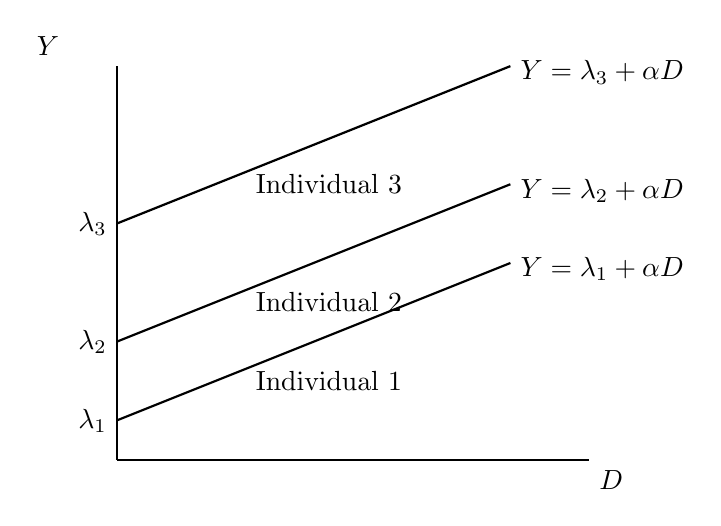
\begin{tikzpicture}[comment/.style={rectangle, text centered}]
			\centering
			\draw [thick] (0,0) -- (6,0) node[anchor=north west] {$D$};
			\draw [thick] (0,0) -- (0,5) node[anchor=south east, xshift=-0.6cm](Y) {$Y$};
			%\node [comment, below of = Y, yshift=0.3cm] {(outcome)};
			
			
			\draw [thick] (0,0.5) -- (5,2.5) node[anchor=north west, yshift=0.2cm] {$Y=\lambda_{1}+\alpha D$};
			\draw [thick] (0,1.5) -- (5,3.5) node[anchor=north west, yshift=0.2cm] {$Y=\lambda_{2}+\alpha D$};
			\draw [thick] (0,3) -- (5,5) node[anchor=north west, yshift=0.2cm] {$Y=\lambda_{3}+\alpha D$};
			
			
			\draw (0,0.5)--(0,0.5) node[anchor=east](Individual 1){$\lambda_{1}$};
			\draw (0,1.5)--(0,1.5) node[anchor=east](Individual 2){$\lambda_{2}$};
			\draw (0,3)--(0,3) node[anchor=east](Individual 3){$\lambda_{3}$};
			
			\draw [comment] node[right of= Individual 1, xshift=2cm, yshift=0.5cm]{Individual 1};
			\draw [comment] node[right of= Individual 2, xshift=2cm, yshift=0.5cm]{Individual 2};
			\draw [comment] node[right of= Individual 3, xshift=2cm, yshift=0.5cm]{Individual 3};
		\end{tikzpicture}
	\end{figure}
	%Recall that shifts in the intercept can be represented using binary regressors,...
\end{frame}





\begin{frame}{Regression with `N-1 dummy variables"}
	\begin{itemize} 
		\item Since regression with `N-1 dummy variables" and regression with fixed effects are the same
		\vspace{0.2cm}
		\item Thus, when there are not many groups (e.g. state, year, county), we usually control these fixed effects by simply including many dummy variables
	\end{itemize}
\end{frame}





\begin{frame}{Fixed Effects Regression}{General Form}
	\begin{itemize} 
		\item We can include many types of fixed effects to control for all possible time-invariant confounding factors or common time factors 
		\begin{equation*}
			Y_{ist}=\lambda_{i}+ \theta_{t} + \kappa_{s} + \alpha D_{ist}+X'_{ist}\beta+\varepsilon_{ist},
		\end{equation*}
		\begin{itemize}
			
			\item $\lambda_{i}$ is called a ``individual fixed effect" or ``individual effect" 
			\vspace{0.2cm}
						\begin{itemize}
				\item It is the constant (fixed) effect of being in individual $i$
				\vspace{0.2cm}
				\item Example: ability or preference
										\vspace{0.2cm}
			\end{itemize}
			\item $\kappa_{s}$ is called a ``state fixed effect" or ``state effect" 
						\vspace{0.2cm}
					\begin{itemize}
			\item It is the constant (fixed) effect of being in state $s$
			\vspace{0.2cm}
						\item Example: culture or geographical features
									\vspace{0.2cm}
					\end{itemize}
			\item $\theta_{t}$ is called a ``year fixed effect" or ``year effect" 
			\vspace{0.2cm}
								\begin{itemize}
			\item It is the constant (fixed) effect of being in year $t$
			\vspace{0.2cm}
			\item Example: business cycle or general time trend
					\end{itemize}
		\end{itemize}
		%\vspace{0.2cm}
		%\item If there are not many fixed effects, we can control these fixed effects by simply including group dummies
	\end{itemize}
\end{frame}



\title[]  
{STATA Example}


\author 
{}

%\institute{Institute of Economics, Academia Sinica  \\ Econ, NTU}
%\institute{Institute of Economics, Academia Sinica  \\ IMES/IDAS, NCCU}
\institute{}

%\author 
%{楊子霆 \\ 中研院經濟所}

%\institute 
%{中正大學國際經濟專題研討}




\date
{}


\begin{frame}{}
	\titlepage
\end{frame}




\begin{frame}{STATA Example}{Data and Code}
	\begin{itemize}
		\item See \textbf{fixed\_effects.do}
		\vspace{0.2cm}
		\item Use cps\_2014\_16.dta
		
		
	\end{itemize}
\end{frame}




\begin{frame}[fragile]{STATA Command: regress}{}
	\item Example:	
\begin{lstlisting}
regress incwage college i.statefip i.year, vce(robust)
\end{lstlisting}
	\begin{itemize}
		\item You can simply use \textbf{regress} by including several sets of dummy variables to get fixed effects estimation
		
	\end{itemize}
	
	
\end{frame}



\begin{frame}[fragile]{STATA Command: areg}{}
	\item Syntax:	
\begin{lstlisting}
areg depvar [indepvars] [if] [in] [weight], absorb(varname) [options]
\end{lstlisting}
	
	\item Example:	
\begin{lstlisting}
areg incwage college i.year, absorb(statefip) vce(robust)
\end{lstlisting}	
\begin{itemize}
	\item \textbf{areg}: Implement regressions with one level of fixed effects
			\vspace{0.2cm}
	\item \textbf{absorb(varname)}: Specifies the categorical variable, which is to be included in the regression as if it were specified by dummy variables
		\vspace{0.2cm}
	\item Note that \textbf{areg} can only include one fixed effect using \textbf{absorb(varname)}
		\vspace{0.2cm}
	\item For other types of fixed effects, you need to include dummy variables by yourself
	
\end{itemize}

	
\end{frame}




\begin{frame}[fragile]{STATA Command: reghdfe}{}
	\begin{itemize}	
	\item To include many levels of fixed effects, we can use this new command \textbf{reghdfe}
\begin{lstlisting}
ssc install reghdfe
\end{lstlisting}

\item For more details, please visit this website: \url{http://scorreia.com/software/reghdfe/index.html}
		
	\end{itemize}
	
	
\end{frame}







\begin{frame}[fragile]{STATA Command: reghdfe}{}
	\item Syntax:	
\begin{lstlisting}
reghdfe depvar [indepvars] [if] [in] [weight] , absorb(absvars) [options]
\end{lstlisting}
	
	\item Example:	
\begin{lstlisting}
reghdfe incwage college, absorb(statefip year) vce(robust)
\end{lstlisting}	
	\begin{itemize}
		\item \textbf{reghdfe}: Implement regressions with many levels of fixed effects
		\vspace{0.2cm}
		\item \textbf{absorb(varname)}: Specifies the categorical variable, which is to be included in the regression as if it were specified by dummy variables
		\vspace{0.2cm}
		\item Note that \textbf{reghdfe} can include many level of fixed effects using \textbf{absorb(varname)}
	
		
	\end{itemize}
	
	
\end{frame}



\begin{frame}[fragile]{STATA Command: outreg2}{Display your results}
	\item Syntax:
\begin{lstlisting}
outreg2 using filename, [options]
\end{lstlisting}
	
	\item Example:
\begin{lstlisting}
reghdfe incwage college age age_sq i.sex i.race, absorb(statefip year) vce(robust)
outreg2 using results.csv, replace keep(college) ///
stats(coef se) addstat(Sample Size, e(N)) ///
addtext(Age, Yes, Sex, Yes, Race, Yes, State FE, Yes, Year FE, Yes)
\end{lstlisting}
	
	\begin{itemize}
		\item \textbf{outreg2}: Outputs regression results to a file (e.g., .csv, .tex)
		\vspace{0.2cm}
		\item \textbf{using results.csv}: Specifies the output file name
		\vspace{0.2cm}
		\item \textbf{keep(college)}: Includes only the coefficient for the variable \texttt{college}
		\vspace{0.2cm}
		\item \textbf{stats(coef se)}: Displays coefficients and standard errors
		
	\end{itemize}
\end{frame}


\begin{frame}[fragile]{STATA Command: outreg2}{Display your results}
	\item Syntax:
\begin{lstlisting}
outreg2 using filename, [options]
\end{lstlisting}

\item Example:
\begin{lstlisting}
reghdfe incwage college age age_sq i.sex i.race, absorb(statefip year) vce(robust)
outreg2 using results.csv, replace keep(college) ///
stats(coef se) addstat(Sample Size, e(N)) ///
addtext(Age, Yes, Sex, Yes, Race, Yes, State FE, Yes, Year FE, Yes)
\end{lstlisting}
	
	\begin{itemize}
	
		\item \textbf{addstat()}: Adds custom statistics, such as sample size
		\vspace{0.2cm}
		\item \textbf{addtext()}: Appends a row with information on controls and fixed effects
	\end{itemize}
\end{frame}




\title[]
{R Example}

\author
{}

%\institute{Institute of Economics, Academia Sinica  \\ Econ, NTU}
%\institute{Institute of Economics, Academia Sinica  \\ IMES/IDAS, NCCU}
\institute{}

%\author
%{Yang Tzu-Ting \\ Institute of Economics, Academia Sinica}

%\institute
%{National Chengchi University, International Economics Seminar}

\date
{}

\begin{frame}{}
	\titlepage
\end{frame}

\begin{frame}{R Example}{Data and Code}
	\begin{itemize}
		\item See \textbf{fixed\_effects.R}
		\vspace{0.2cm}
		\item Use cps\_2014\_16.dta
	\end{itemize}
\end{frame}

\begin{frame}[fragile]{R Command: lm() for Fixed Effects}{}
	\item Example:
\begin{lstlisting}[language=R]
library(dplyr)

# Load data
data <- read_dta(paste0(rawdata, "/cps_2014_16.dta"))


# Fit the model with state and year fixed effects using dummy variables
model <- lm(incwage ~ college + factor(statefip) + factor(year), data = data)
summary(model)
\end{lstlisting}
	\begin{itemize}
		\item You can use \texttt{lm()} with dummy variables to estimate fixed effects
		\vspace{0.2cm}
		\item Here, \texttt{factor()} is used to include categorical variables as fixed effects in the model
	\end{itemize}
\end{frame}









\begin{frame}[fragile]{R Command: plm() for Fixed Effects}{}
	\item Example:
\begin{lstlisting}[language=R]
library(plm)

# Convert to panel data
pdata <- pdata.frame(data, index = c("statefip", "year"))

# Fixed effects model using plm
model_fe <- plm(incwage ~ college, data = pdata, model = "within")
summary(model_fe)
\end{lstlisting}
	\begin{itemize}
		\item \texttt{plm()}: Implements regressions with one level of fixed effects (e.g., individual or time)
		\vspace{0.2cm}
		\item \texttt{model = "within"}: Specifies that fixed effects are to be used
		\vspace{0.2cm}
		\item \texttt{pdata.frame()}: Converts the data to a panel data frame, which is required by \texttt{plm}
	\end{itemize}
\end{frame}

\begin{frame}[fragile]{R Command: fixest for High-Dimensional Fixed Effects}{}

\begin{lstlisting}[language=R]
library(fixest)

# Fixed effects regression with multiple controls and fixed effects
model_hdfe <- feols(incwage ~ college + age + age_sq + 
factor(sex) + factor(race) | 
statefip + year, 
data = data, vcov = "hetero")

summary(model_hdfe)
\end{lstlisting}
	\begin{itemize}
		\item \textbf{feols()}: Performs linear regression with support for high-dimensional fixed effects
		\vspace{0.2cm}
			\begin{itemize}
		\item Fixed effects are specified after the \texttt{|} symbol, e.g., \texttt{statefip + year}
		\vspace{0.2cm}
		\item \textbf{vcov = "hetero"}: Computes heteroskedasticity-robust standard errors
			\end{itemize}
	\end{itemize}
\end{frame}



\begin{frame}[fragile]{R Command: modelsummary for Regression Output}
	
	\vspace{0.3cm}
\begin{lstlisting}[language=R]
modelsummary(
models,
coef_omit = "^(?!college)",       # Keep only 'college'
statistic = "std.error",          # Show robust SEs
gof_map = c("nobs" = "Sample Size"),  # Rename N
notes = notes,                    # Add notes per model
output = file.path(workdata, "results.csv")  # Save output
)
\end{lstlisting}
	

\end{frame}






\end{document} 